\chapter{System Analysis}
\label{chap:system_analysis}

\section{Requirement Analysis}
\label{sec:sys_req_analysis}

The architectural specification of ChronaNexus is guided by three converging domains of requirements: clinical safety imperatives, regulatory compliance frameworks, and computational feasibility within resource-constrained healthcare environments.

\subsection{Clinical Safety Imperatives}
In healthcare decision support, false positive assertions (e.g., falsely asserting that a patient's kidney function is normal when serum creatinine is elevated) and false negative omissions (e.g., failing to surface a severe penicillin allergy recorded four years prior) carry life-threatening consequences. Traditional conversational language models optimize for linguistic fluency rather than factual entailment. Consequently, the primary clinical safety requirement is \textbf{fail-closed operation}: whenever retrieved evidence is ambiguous, incomplete, or mathematically inconsistent, the system must deterministically withhold unverified clinical assertions, emit cautionary notices, and prompt the clinician for manual verification.

\subsection{Regulatory Compliance and Data Sovereignty}
Under emerging healthcare data protection frameworks---including India's Digital Personal Data Protection (DPDP) Act 2023 and the Ayushman Bharat Digital Mission (ABDM) sandbox standards~\cite{nha2022abdm}---patient health records constitute sensitive personal data. The system must enforce:
\begin{enumerate}
    \item \textbf{Data Sovereignty}: Sensitive patient-identifiable clinical records must remain stored within local clinic boundaries or encrypted private storage, preventing unencrypted data transmission to external public cloud APIs.
    \item \textbf{Cryptographic Tamper-Evidence}: Every ingested medical document must be hashed via SHA-256 to ensure data provenance and detect unauthorized record alteration.
    \item \textbf{Granular Auditability}: Every generated clinical statement must maintain verifiable bi-directional provenance, linking assertions directly to the source document hash, page index, and exact textual chunk.
\end{enumerate}

\subsection{Operational Feasibility in Tier-2 and Rural Clinics}
Community healthcare centers and outpatient dispensaries frequently operate on modest desktop workstations without dedicated GPU accelerators. ChronaNexus must therefore support a dual-execution paradigm: operating primarily on lightweight local Small Language Models (SLMs) running on standard x86 CPU hardware ($<4\text{ GB}$ system RAM) via Ollama, while retaining seamless fallback to cloud APIs (such as Groq) when high-throughput batch summarization is required.


\section{Stakeholder and Actor Profiles}
\label{sec:sys_stakeholders}

The platform interacts with four distinct human and organizational personas. Table~\ref{tab:3_1_stakeholders} outlines their profiles, responsibilities, and operational system touchpoints.

\small
\begin{longtable}{@{}p{0.18\linewidth} p{0.24\linewidth} p{0.28\linewidth} p{0.22\linewidth}@{}}
\caption{Stakeholder profiles and operational touchpoints}\label{tab:3_1_stakeholders} \\
\toprule
\textbf{Stakeholder Role} & \textbf{Persona Description} & \textbf{Operational Responsibility} & \textbf{Core Touchpoint} \\
\midrule
\endfirsthead
\toprule
\multicolumn{4}{c}{\small\textit{Stakeholder profiles and touchpoints (Continued)}} \\[4pt]
\midrule
\textbf{Stakeholder Role} & \textbf{Persona Description} & \textbf{Operational Responsibility} & \textbf{Core Touchpoint} \\
\midrule
\endhead
\midrule
\multicolumn{4}{r}{\footnotesize\textit{Continued on next page...}} \\
\bottomrule
\endfoot
\bottomrule
\endlastfoot
\textbf{Patient / Family} & Individual managing chronic illness or longitudinal medical history. & Uploads historical documents; queries trends; uses multilingual voice assistant; triggers SOS in crisis. & Patient Web Portal, Multilingual Voice UI, Emergency SOS Button. \\
\midrule
\textbf{Attending Clinician} & Medical practitioner conducting acute or routine outpatient consultations. & Reviews synthesized multi-year timeline; evaluates lab delta trends; verifies medication lists in $<5\text{ min}$. & Clinician Dashboard, Longitudinal Timeline, Dynamic Lab Charts. \\
\midrule
\textbf{Clinical Auditor} & Quality compliance officer or senior physician auditing AI decisions. & Audits claim-context grounding; inspects verification logs; evaluates citation precision and benchmark fidelity. & Verification Audit Log, Provenance Inspector, Citation Badges. \\
\midrule
\textbf{108 Emergency Dispatcher} & Municipal ambulance coordinator or paramedic dispatch officer. & Receives automated JSON triage payload (blood group, critical allergies, recent vitals, GPS coordinates). & Emergency Dispatch Webhook, Triage JSON Stream, Map Locator. \\
\bottomrule
\end{longtable}
\normalsize


\section{Use Case Modeling and Scenarios}
\label{sec:sys_use_cases}

The behavioral requirements of ChronaNexus are formally modeled through UML use cases. Figure~\ref{fig:3_1_usecase} depicts the primary actors, system boundary, and core use cases, including the critical \texttt{<<includes>>} dependency between clinical question-answering and evidence verification.

\begin{figure}[htbp]
    \centering
    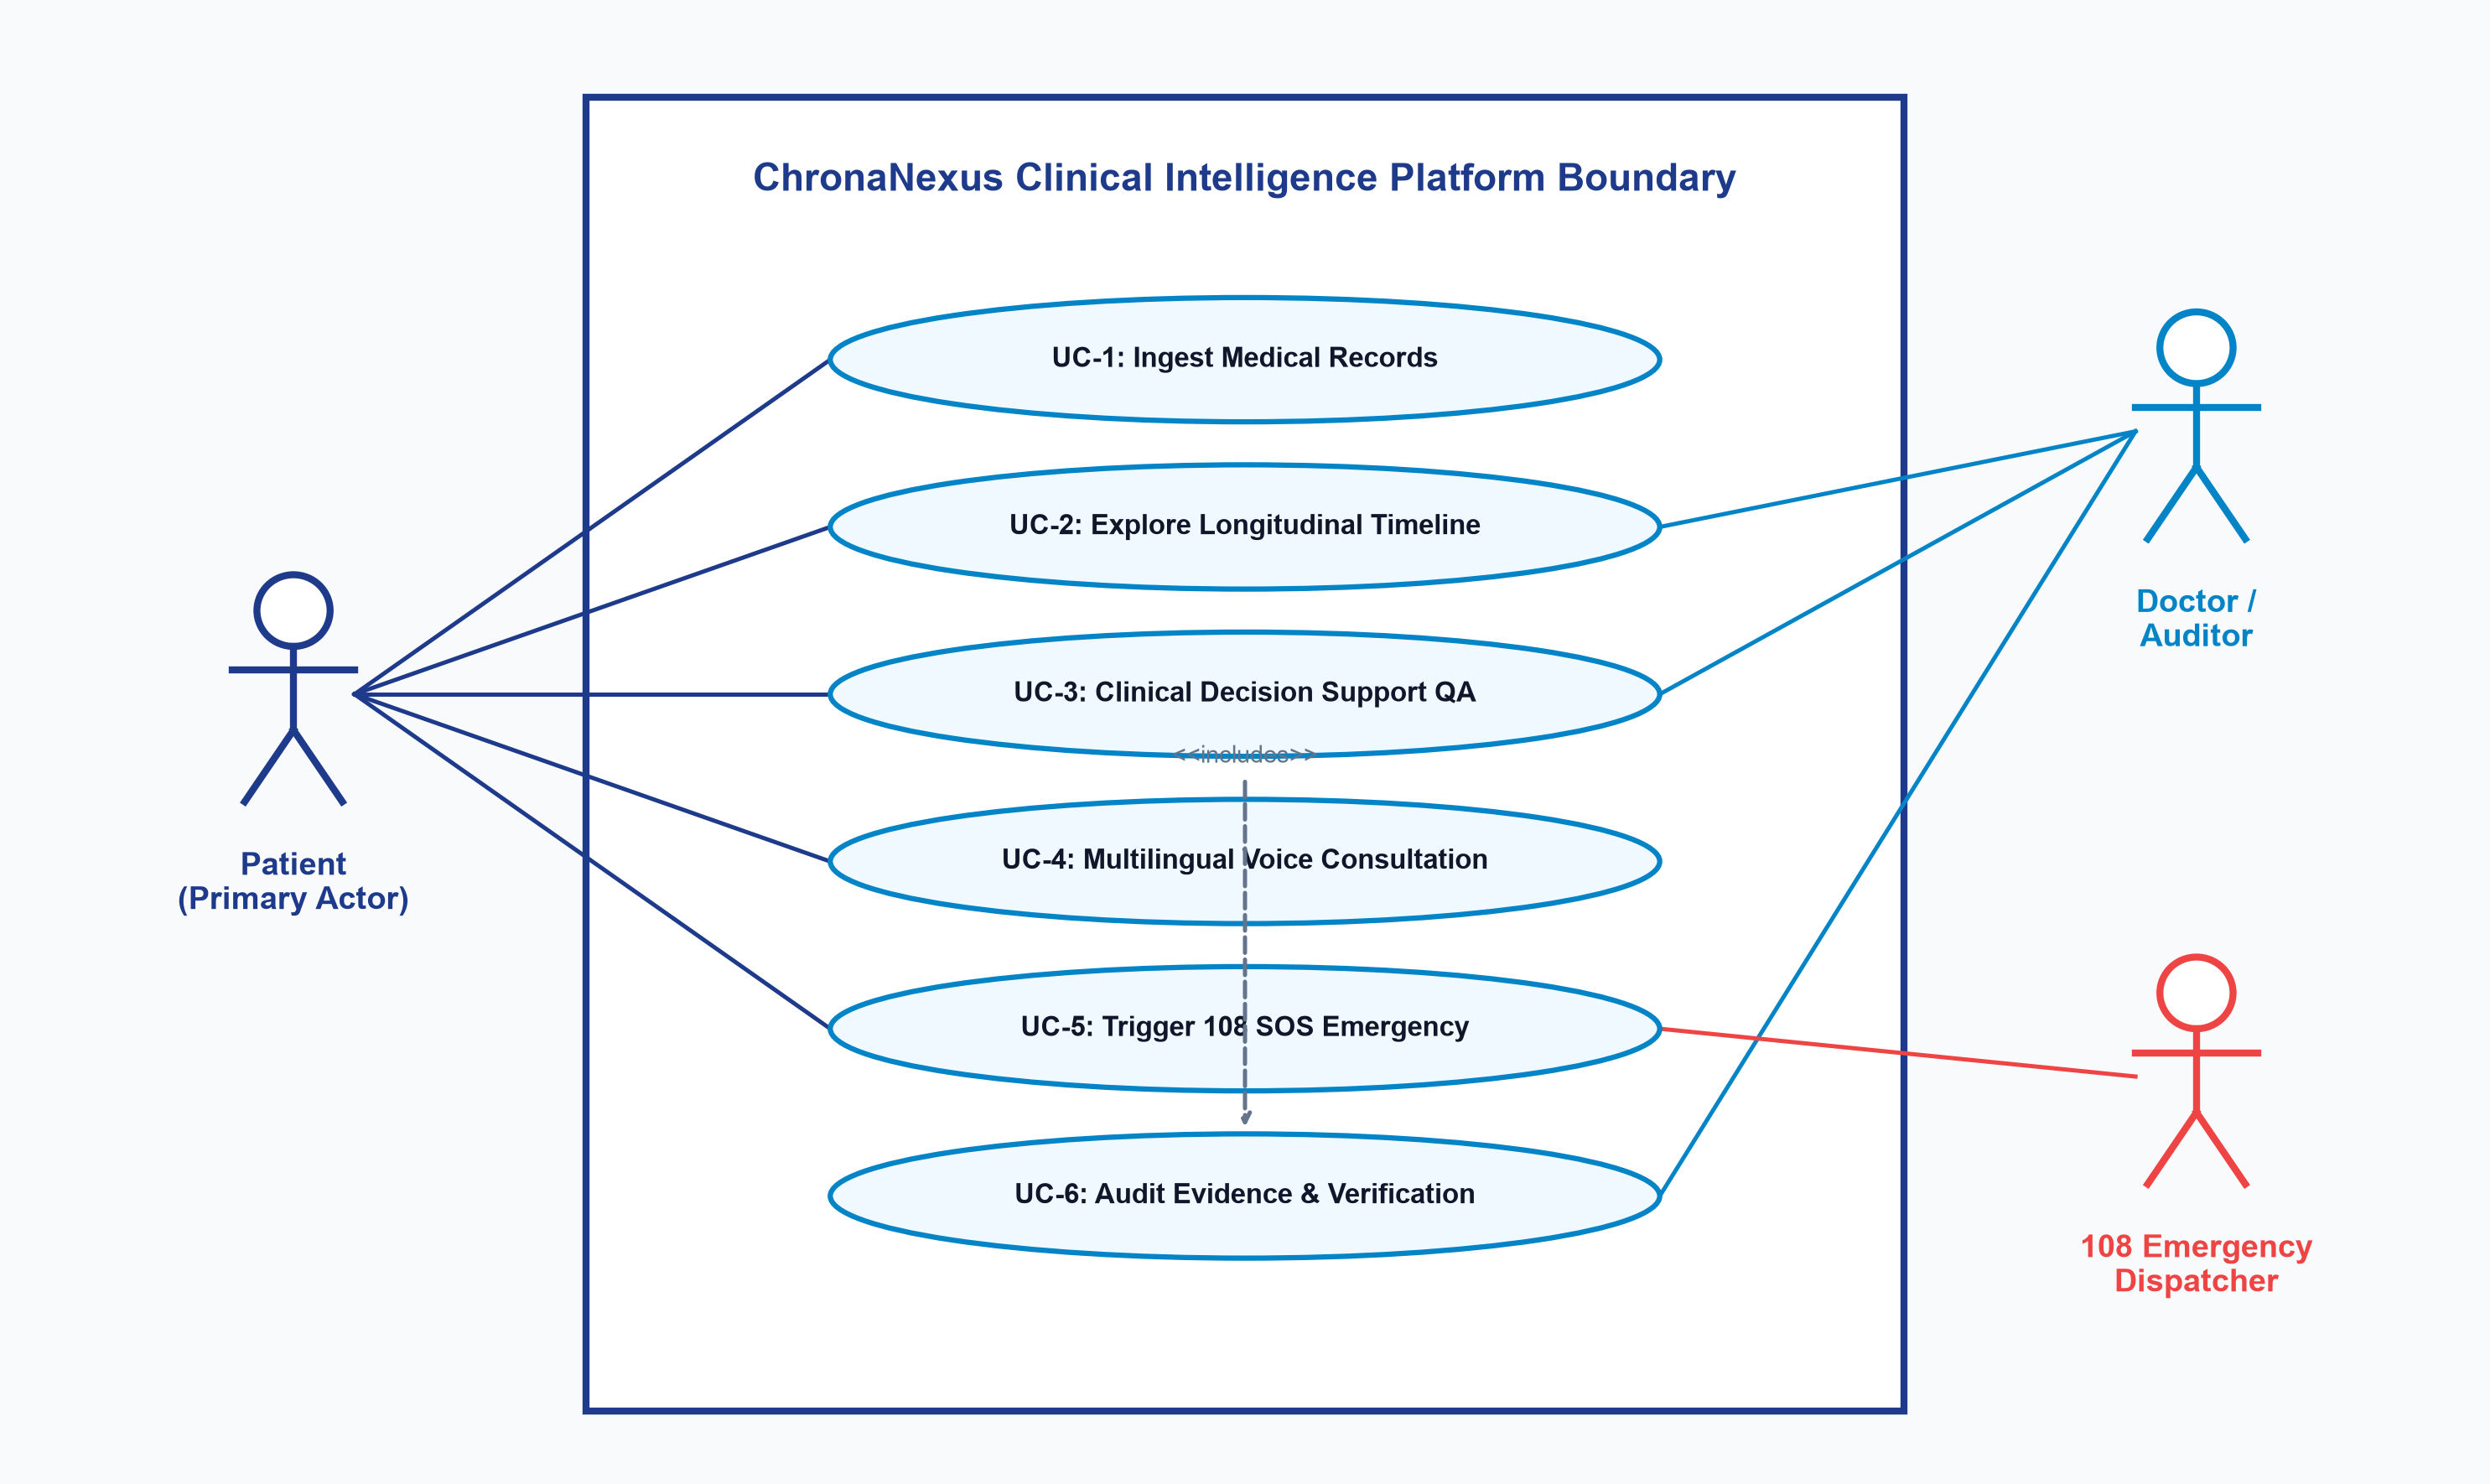
\includegraphics[width=0.95\linewidth]{figures/fig3_1_usecase.png}
    \caption{ChronaNexus UML Use Case Diagram illustrating primary actors and system capabilities.}
    \label{fig:3_1_usecase}
\end{figure}

The functional interactions within the platform are formalized through six core use cases:

\subsection{UC-1: Ingest and Extract Longitudinal Medical Records}
\begin{itemize}
    \item \textbf{Primary Actor}: Patient, Hospital Records Staff.
    \item \textbf{Preconditions}: User is authenticated; uploaded artifact is a valid PDF or image ($<25\text{ MB}$).
    \item \textbf{Trigger}: User selects and uploads a batch of clinical lab reports or prescriptions.
    \item \textbf{Main Success Scenario}:
    \begin{enumerate}
        \item System computes SHA-256 binary hash and checks database for duplicate files.
        \item \texttt{PyMuPDF} extracts raw text and spatial bounding boxes of unruled tables.
        \item Clinical terminology normalizer maps entities to LOINC and RxNorm catalogs.
        \item Records are ingested into the relational database and vectorized into ChromaDB.
        \item System confirms successful upload and updates the longitudinal timeline.
    \end{enumerate}
    \item \textbf{Postconditions}: Document is indexed; structured records are queryable.
\end{itemize}

\subsection{UC-2: Explore Synthesized Longitudinal Clinical Timeline}
\begin{itemize}
    \item \textbf{Primary Actor}: Clinician, Patient.
    \item \textbf{Preconditions}: At least one processed clinical encounter exists in the patient profile.
    \item \textbf{Trigger}: User navigates to the Patient Timeline view.
    \item \textbf{Main Success Scenario}:
    \begin{enumerate}
        \item System executes an indexed SQL query ordering encounters chronologically (2019--2026).
        \item Structured lab trends are aggregated to compute historical deltas (e.g., HbA1c trajectory).
        \item Timeline components render interactive visual cards with date, facility, and provider.
    \end{enumerate}
    \item \textbf{Postconditions}: User inspects multi-year progression without manual document review.
\end{itemize}

\subsection{UC-3: Interactive Clinical Decision Support Question-Answering}
\begin{itemize}
    \item \textbf{Primary Actor}: Clinician, Patient.
    \item \textbf{Preconditions}: Ingestion complete; local SLM or cloud LLM backend is active.
    \item \textbf{Trigger}: User enters a natural language inquiry (e.g., \textit{"What is my latest Fasting Glucose reading and how has it changed?"}).
    \item \textbf{Main Success Scenario}:
    \begin{enumerate}
        \item Query router determines whether inquiry requires structured SQL aggregation or RAG.
        \item Dual-channel retriever fetches candidate chunks via dense BGE embeddings and BM25 Okapi.
        \item Reciprocal Rank Fusion ($k=60$) merges results; top-5 passages are passed to language model.
        \item Model generates draft response conditioned strictly on retrieved evidence.
        \item System invokes UC-6 to verify claims before returning final response with citation badges.
    \end{enumerate}
    \item \textbf{Postconditions}: Grounded, audited response displayed with clickable chunk references.
\end{itemize}

\subsection{UC-4: Multilingual Voice Consultation via Indic Phonetic Bridge}
\begin{itemize}
    \item \textbf{Primary Actor}: Patient.
    \item \textbf{Preconditions}: Microphone enabled; target language selected (e.g., Odia).
    \item \textbf{Trigger}: Patient clicks the voice consultation microphone button and speaks inquiry.
    \item \textbf{Main Success Scenario}:
    \begin{enumerate}
        \item Browser captures speech and converts audio to text in target language.
        \item Backend processes query via UC-3 and generates verified clinical response text.
        \item For Odia speech, the Unicode phonetic bridge maps codepoints ($\Delta = -0x0180$) to Bengali.
        \item Microsoft Edge Neural TTS streams high-prosody audio back to frontend player ($<1.5\text{ s}$).
    \end{enumerate}
    \item \textbf{Postconditions}: Patient hears natural native-cadence response in selected language.
\end{itemize}

\subsection{UC-5: Trigger Emergency SOS Triage \& Hospital Discovery}
\begin{itemize}
    \item \textbf{Primary Actor}: Patient, Caregiver.
    \item \textbf{Preconditions}: Browser geolocation permission granted; emergency profile saved.
    \item \textbf{Trigger}: User clicks the red Emergency SOS button.
    \item \textbf{Main Success Scenario}:
    \begin{enumerate}
        \item System retrieves critical medical summary: blood group, allergies, active medications.
        \item System captures user coordinates and queries OpenStreetMap Overpass API.
        \item Emergency centers within $10\text{ km}$ are ranked via Haversine distance formula.
        \item Structured triage JSON payload is generated for 108 ambulance dispatch integration.
    \end{enumerate}
    \item \textbf{Postconditions}: Nearest hospitals displayed with routing; dispatch payload ready.
\end{itemize}

\subsection{UC-6: Audit Evidence Grounding and Citation Verification}
\begin{itemize}
    \item \textbf{Primary Actor}: System Kernel (Included by UC-3), Clinical Auditor.
    \item \textbf{Preconditions}: Candidate LLM response generated alongside retrieved passages.
    \item \textbf{Main Success Scenario}:
    \begin{enumerate}
        \item Claim extractor decomposes draft response into atomic proposition statements.
        \item Tier 1 symbolic rule engine matches numerical readings, dates, and dosages ($<5\text{ ms}$).
        \item Unresolved claims pass to Tier 2 neural natural language inference cross-encoder.
        \item Claims failing verification are retracted or marked with cautionary warning flags.
        \item Audit record is logged in database with entailment score, chunk ID, and verdict.
    \end{enumerate}
    \item \textbf{Postconditions}: Response achieves $100\%$ citation attribution precision on evidence.
\end{itemize}


\section{Dynamic Behavioral Modeling: UML Activity Diagram}
\label{sec:sys_activity}

To replace dense textual procedures with formal graphical execution flows, Figure~\ref{fig:3_2_activity} presents the UML Activity Diagram for the multi-modal clinical query and document ingestion lifecycle. Architectural responsibilities are structured across four swimlanes: the user actor, the frontend and API gateway, the clinical processing pipeline, and the persistence stores.

\begin{figure}[htbp]
    \centering
    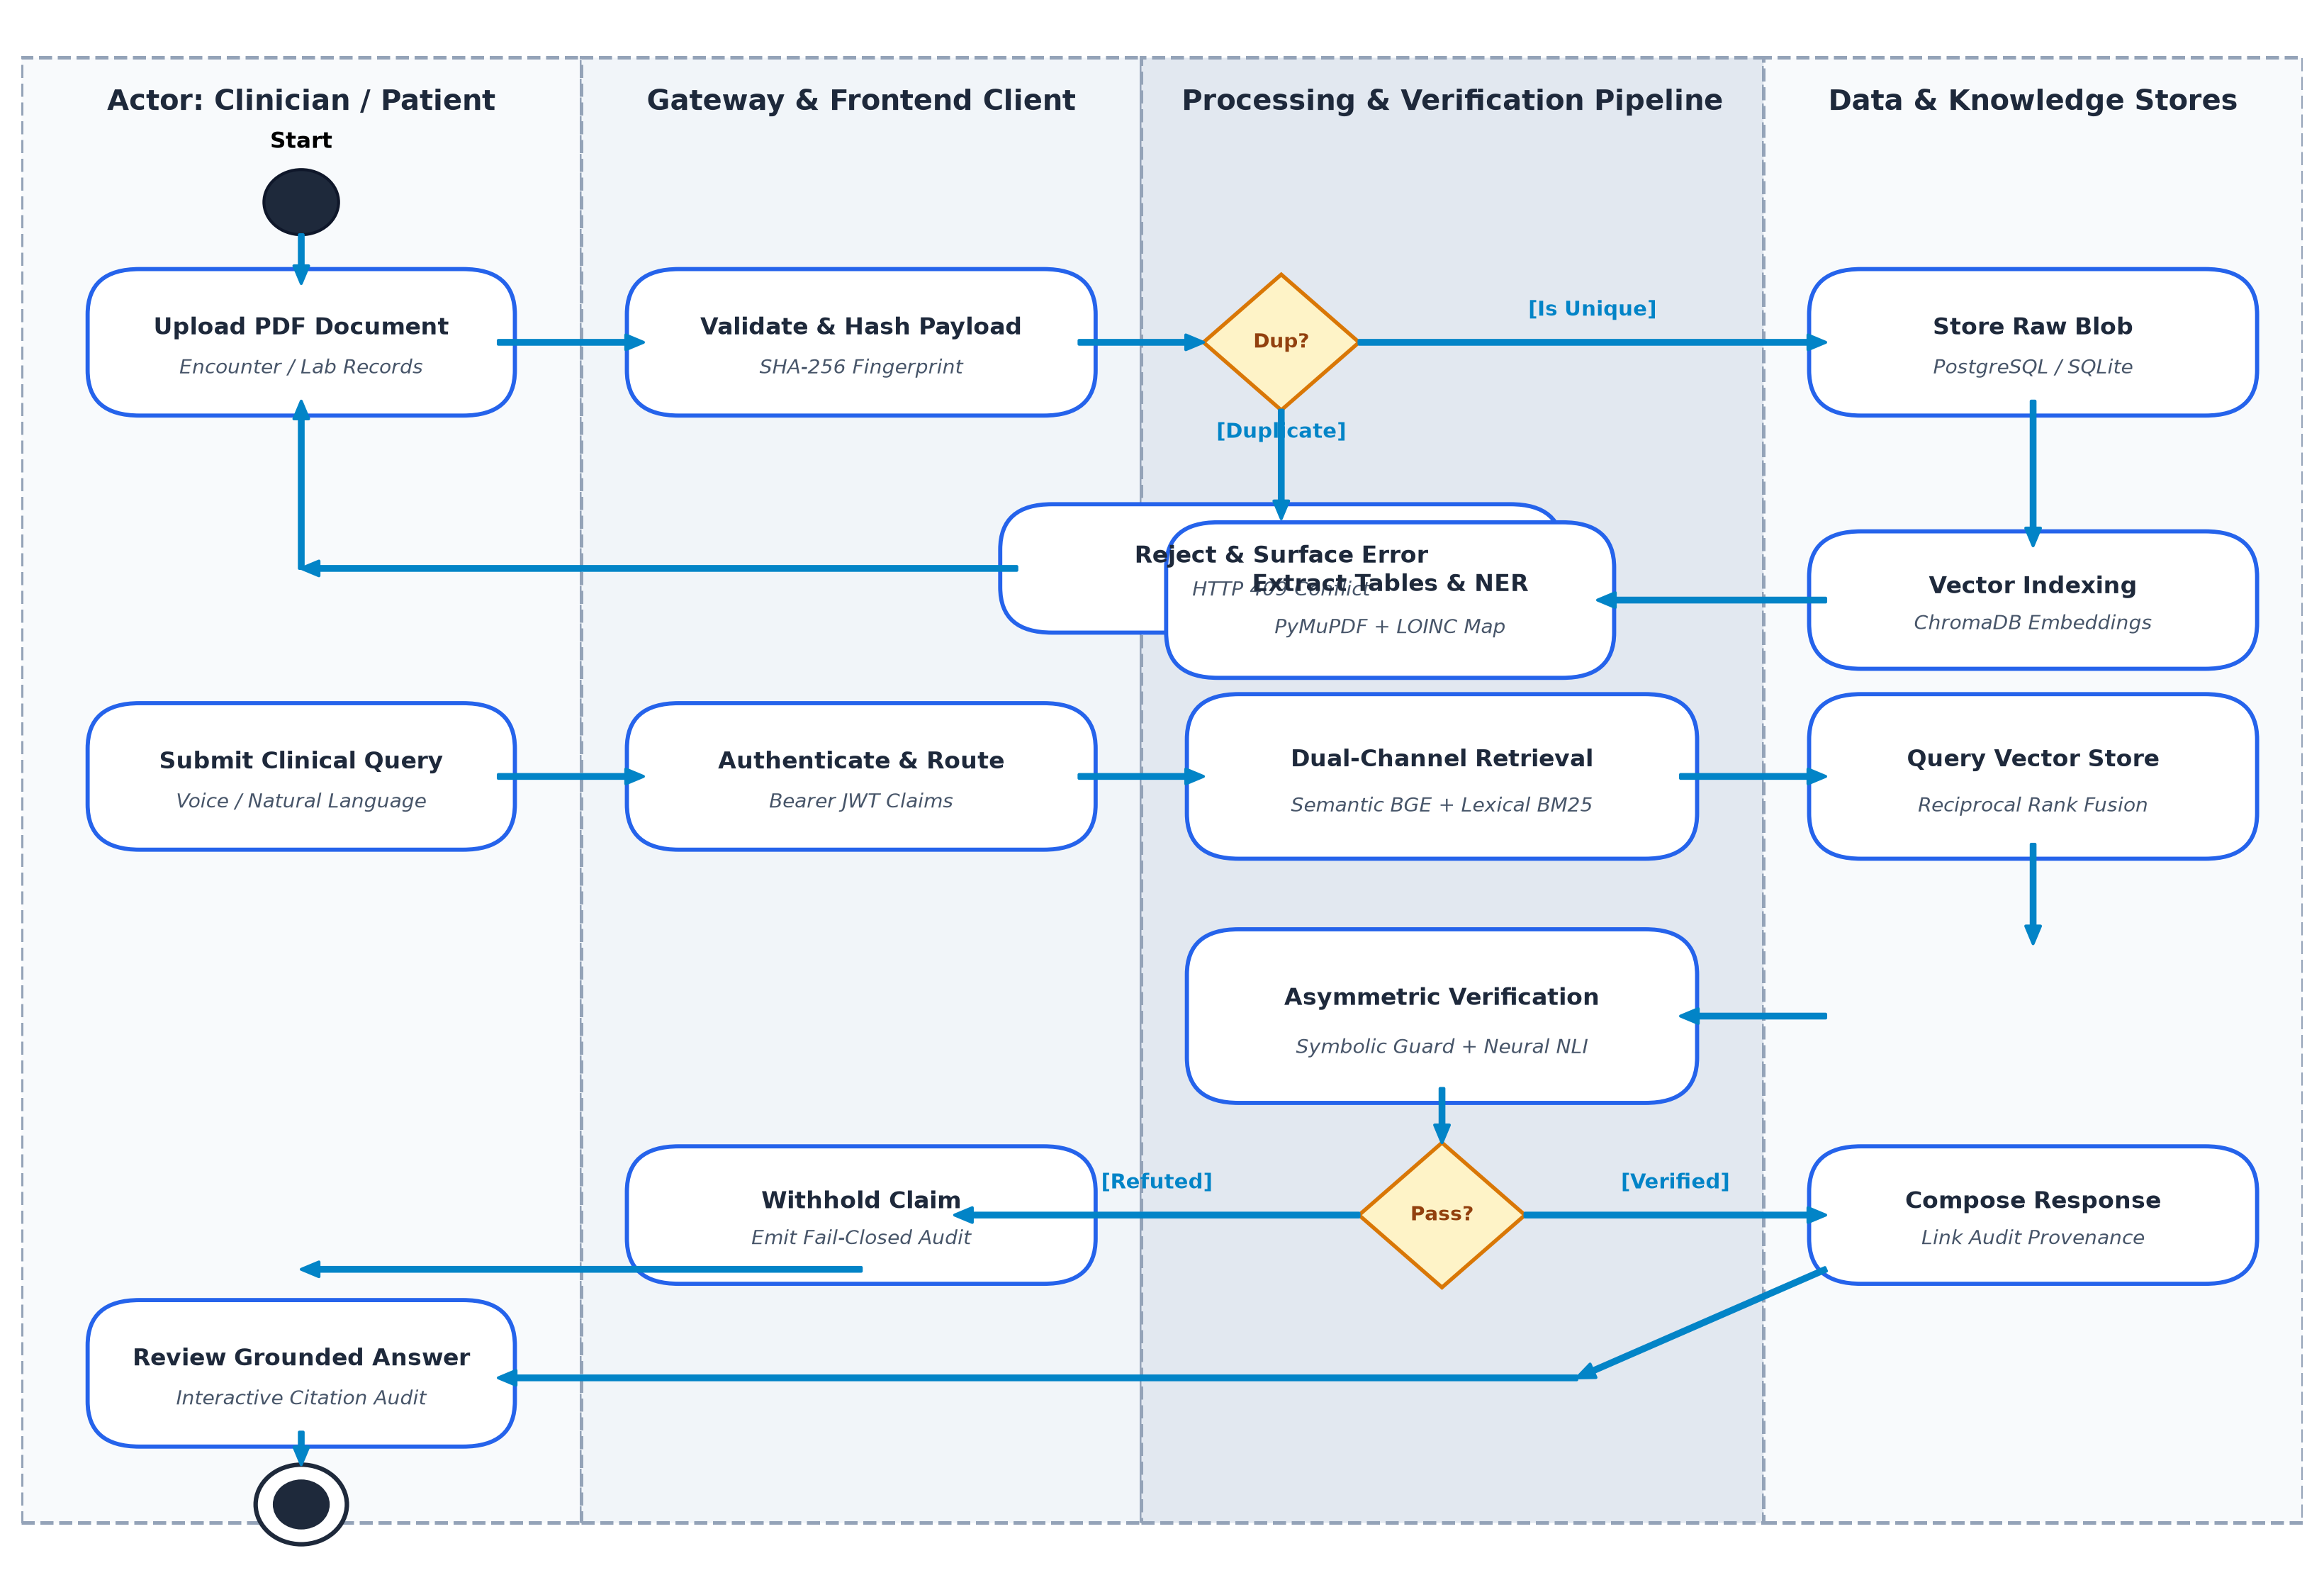
\includegraphics[width=0.95\linewidth]{figures/fig3_2_activity.png}
    \caption{ChronaNexus UML Activity Diagram delineating parallel ingestion, dual-channel retrieval, and fail-closed claim verification across architectural swimlanes.}
    \label{fig:3_2_activity}
\end{figure}

The diagram formalizes the operational decision flow:
\begin{enumerate}
    \item \textbf{Ingestion Branch}: Uploaded PDF documents are hashed via SHA-256. A decision diamond evaluates whether the document already exists in the database. Duplicates are immediately rejected with HTTP 409, while unique files proceed in parallel to relational blob storage, LOINC entity normalization, and ChromaDB vector indexing.
    \item \textbf{Query and Verification Flow}: Natural language queries trigger dual-channel lexical (BM25) and semantic (BGE) retrieval. Candidate clinical assertions enter the asymmetric verification engine.
    \item \textbf{Decision Outcome}: The decision guard evaluates whether the claim meets the grounding threshold ($F_1 \ge 0.85$). Passing claims are synthesized into a grounded response with citations; failing claims branch into a fail-closed withholding state that logs an audit record and surfaces a cautionary disclaimer.
\end{enumerate}


\section{Functional Requirements}
\label{sec:sys_functional_reqs}

The functional capabilities of ChronaNexus are categorized into four core operational subsystems, formalizing requirements FR-01 through FR-16 in Tables~\ref{tab:3_2_vault_reqs} through~\ref{tab:3_5_voice_reqs}.

\small
\begin{longtable}{@{}p{0.16\linewidth} p{0.31\linewidth} p{0.45\linewidth}@{}}
\caption{Document vault and medical understanding functional requirements}\label{tab:3_2_vault_reqs} \\
\toprule
\textbf{Requirement ID} & \textbf{Requirement Title} & \textbf{Technical Specification} \\
\midrule
\endfirsthead
\toprule
\multicolumn{3}{c}{\small\textit{Document vault requirements (Continued)}} \\[4pt]
\midrule
\textbf{Requirement ID} & \textbf{Requirement Title} & \textbf{Technical Specification} \\
\midrule
\endhead
\midrule
\multicolumn{3}{r}{\footnotesize\textit{Continued on next page...}} \\
\bottomrule
\endfoot
\bottomrule
\endlastfoot
\textbf{FR-01} & Multi-Format Ingestion & Ingest native and scanned medical PDFs up to $25\text{ MB}$, verifying MIME type and structure. \\
\midrule
\textbf{FR-02} & SHA-256 Deduplication & Compute cryptographic hash; reject duplicate uploads and maintain file-level integrity. \\
\midrule
\textbf{FR-03} & Spatial Table Extraction & Detect unruled laboratory tables via \texttt{PyMuPDF}, normalizing rows into structured markdown. \\
\midrule
\textbf{FR-04} & Terminology Mapping & Normalize extracted clinical entities to canonical LOINC, RxNorm, and ICD-10 ontologies. \\
\bottomrule
\end{longtable}
\normalsize

\small
\begin{longtable}{@{}p{0.16\linewidth} p{0.31\linewidth} p{0.45\linewidth}@{}}
\caption{Timeline and structured query engine functional requirements}\label{tab:3_3_timeline_reqs} \\
\toprule
\textbf{Requirement ID} & \textbf{Requirement Title} & \textbf{Technical Specification} \\
\midrule
\endfirsthead
\toprule
\multicolumn{3}{c}{\small\textit{Timeline requirements (Continued)}} \\[4pt]
\midrule
\textbf{Requirement ID} & \textbf{Requirement Title} & \textbf{Technical Specification} \\
\midrule
\endhead
\midrule
\multicolumn{3}{r}{\footnotesize\textit{Continued on next page...}} \\
\bottomrule
\endfoot
\bottomrule
\endlastfoot
\textbf{FR-05} & Chronological Synthesis & Assemble multi-year patient records (2019--2026) in monotonic chronological order. \\
\midrule
\textbf{FR-06} & Delta Trend Computation & Deterministically compute numerical differences between successive lab tests ($\Delta = V_t - V_{t-1}$). \\
\midrule
\textbf{FR-07} & Conflict Detection & Flag clinical anomalies where conflicting values occur across differing hospital facilities. \\
\midrule
\textbf{FR-08} & Relational SQL Aggregation & Provide instant SQL queries for vitals and lab panels bypassing vector search overhead. \\
\bottomrule
\end{longtable}
\normalsize

\small
\begin{longtable}{@{}p{0.16\linewidth} p{0.31\linewidth} p{0.45\linewidth}@{}}
\caption{Dual-channel hybrid RAG and evidence verification functional requirements}\label{tab:3_4_rag_reqs} \\
\toprule
\textbf{Requirement ID} & \textbf{Requirement Title} & \textbf{Technical Specification} \\
\midrule
\endfirsthead
\toprule
\multicolumn{3}{c}{\small\textit{Hybrid RAG requirements (Continued)}} \\[4pt]
\midrule
\textbf{Requirement ID} & \textbf{Requirement Title} & \textbf{Technical Specification} \\
\midrule
\endhead
\midrule
\multicolumn{3}{r}{\footnotesize\textit{Continued on next page...}} \\
\bottomrule
\endfoot
\bottomrule
\endlastfoot
\textbf{FR-09} & Dense Semantic Retrieval & Generate $384$-dimensional embeddings via \texttt{bge-small-en-v1.5} with cosine similarity. \\
\midrule
\textbf{FR-10} & Lexical Inverted Index & Execute BM25 Okapi token search to preserve exact dosage numbers and pharmaceutical terms. \\
\midrule
\textbf{FR-11} & Reciprocal Rank Fusion & Aggregate dense and lexical rankings via RRF ($k=60$) to construct optimal top-5 context. \\
\midrule
\textbf{FR-12} & 2-Tier Claim Verification & Execute Tier 1 symbolic rule checking ($<5\text{ ms}$) escalated to Tier 2 neural NLI. \\
\midrule
\textbf{FR-13} & Citation Attribution & Affix clickable citation badges to every assertion with document ID and page index. \\
\bottomrule
\end{longtable}
\normalsize

\small
\begin{longtable}{@{}p{0.16\linewidth} p{0.31\linewidth} p{0.45\linewidth}@{}}
\caption{Multilingual voice and emergency dispatch functional requirements}\label{tab:3_5_voice_reqs} \\
\toprule
\textbf{Requirement ID} & \textbf{Requirement Title} & \textbf{Technical Specification} \\
\midrule
\endfirsthead
\toprule
\multicolumn{3}{c}{\small\textit{Voice and dispatch requirements (Continued)}} \\[4pt]
\midrule
\textbf{Requirement ID} & \textbf{Requirement Title} & \textbf{Technical Specification} \\
\midrule
\endhead
\midrule
\multicolumn{3}{r}{\footnotesize\textit{Continued on next page...}} \\
\bottomrule
\endfoot
\bottomrule
\endlastfoot
\textbf{FR-14} & 6-Language Voice Synthesis & Stream synthesized speech across English, Hindi, Odia, Telugu, Tamil, and Bengali. \\
\midrule
\textbf{FR-15} & Indic Unicode Bridge & Transliterate Odia codepoints ($\Delta = -0x0180$) to Bengali for natural prosody Edge TTS. \\
\midrule
\textbf{FR-16} & 108 Emergency Dispatch & Construct automated triage JSON payload with Haversine hospital discovery within $10\text{ km}$. \\
\bottomrule
\end{longtable}
\normalsize


\section{Non-Functional Requirements}
\label{sec:sys_non_functional_reqs}

ChronaNexus adheres to strict non-functional performance benchmarks:
\begin{enumerate}
    \item \textbf{Inference Latency}: Mean query-to-response latency must remain below $1.5\text{ s}$ using cloud LLMs (Groq) and below $3.0\text{ s}$ during fully offline local SLM CPU inference (Ollama). Voice synthesis audio streaming must begin within $1.5\text{ s}$ of generation.
    \item \textbf{System Resource Footprint}: The complete local runtime (FastAPI, SQLite, ChromaDB, and quantized SLM) must execute on standard clinic workstations with $\le 4\text{ GB}$ available RAM without requiring discrete GPU hardware.
    \item \textbf{Verification Accuracy \& Citation Precision}: The hybrid verification engine must achieve $\ge 85\%$ accuracy on multi-assertion clinical benchmarks and $100\%$ citation attribution precision on evaluated context passages.
    \item \textbf{Data Sovereignty \& Privacy}: Protected Health Information (PHI) must never be transmitted unencrypted across public networks. Local-first execution must operate with zero outbound internet traffic.
    \item \textbf{Reliability and Automated Test Coverage}: The software kernel must validate against $190$ automated backend unit and integration tests across $12$ test suites, enforcing active database interception to prevent test pollution of production data.
\end{enumerate}


\section{Requirements Traceability Matrix (RTM)}
\label{sec:sys_rtm}

Table~\ref{tab:3_6_rtm} provides the complete Requirements Traceability Matrix, mapping each functional requirement to its architectural module, verification mechanism, and corresponding test suite.

\small
\begin{longtable}{@{}p{0.12\linewidth} p{0.30\linewidth} p{0.28\linewidth} p{0.22\linewidth}@{}}
\caption{Requirements Traceability Matrix (RTM) linking specifications to implementation and test suites}\label{tab:3_6_rtm} \\
\toprule
\textbf{Req. ID} & \textbf{Functional Feature} & \textbf{Implemented Subsystem} & \textbf{Verified Test Case} \\
\midrule
\endfirsthead
\toprule
\multicolumn{4}{c}{\small\textit{Requirements Traceability Matrix (Continued)}} \\[4pt]
\midrule
\textbf{Req. ID} & \textbf{Functional Feature} & \textbf{Implemented Subsystem} & \textbf{Verified Test Case} \\
\midrule
\endhead
\midrule
\multicolumn{4}{r}{\footnotesize\textit{Continued on next page...}} \\
\bottomrule
\endfoot
\bottomrule
\endlastfoot
\textbf{FR-01} & Multi-Format PDF Ingestion & Document Parser (\texttt{parser.py}) & TC-01 (Parser Suite) \\
\midrule
\textbf{FR-02} & SHA-256 Deduplication & Vault Router (\texttt{documents.py}) & TC-02 (Vault Suite) \\
\midrule
\textbf{FR-03} & Spatial Table Extraction & Table Extractor (\texttt{tables.py}) & TC-03 (Table Suite) \\
\midrule
\textbf{FR-04} & Clinical Terminology Mapping & Normalizer (\texttt{normalizer.py}) & TC-04 (Ontology Suite) \\
\midrule
\textbf{FR-05} & Chronological Synthesis & Timeline Service (\texttt{timeline.py}) & TC-05 (Timeline Suite) \\
\midrule
\textbf{FR-06} & Delta Trend Computation & Query Engine (\texttt{query\_engine.py}) & TC-06 (Trend Suite) \\
\midrule
\textbf{FR-07} & Conflict Detection & Conflict Detector (\texttt{conflicts.py}) & TC-07 (Conflict Suite) \\
\midrule
\textbf{FR-08} & Relational SQL Aggregation & Database Core (\texttt{database.py}) & TC-08 (SQL Engine Suite) \\
\midrule
\textbf{FR-09} & Dense Vector Retrieval & Dense RAG (\texttt{dense\_retriever.py}) & TC-09 (Dense RAG Suite) \\
\midrule
\textbf{FR-10} & BM25 Lexical Matching & BM25 Engine (\texttt{bm25\_retriever.py}) & TC-10 (BM25 Suite) \\
\midrule
\textbf{FR-11} & Reciprocal Rank Fusion & Hybrid Retriever (\texttt{hybrid\_rag.py}) & TC-11 (Hybrid RRF Suite) \\
\midrule
\textbf{FR-12} & 2-Tier Claim Verification & Evidence Verifier (\texttt{verifier.py}) & TC-12 (Verifier Suite) \\
\midrule
\textbf{FR-13} & Clickable Citation Provenance & Chat Router (\texttt{chat.py}) & TC-13 (Citation Suite) \\
\midrule
\textbf{FR-14} & 6-Language Voice Synthesis & Speech Engine (\texttt{tts.py}) & TC-14 (TTS Audio Suite) \\
\midrule
\textbf{FR-15} & Indic Unicode Phonetic Bridge & Indic Transliteration (\texttt{tts.py}) & TC-15 (Indic Bridge Suite) \\
\midrule
\textbf{FR-16} & 108 Emergency Dispatch & Emergency Router (\texttt{emergency.py}) & TC-16 (Dispatch Suite) \\
\bottomrule
\end{longtable}
\normalsize

\newpage
